\section{Lab Assignment 6}
\paragraph{Objective:}

The objective is to assess how different vulnerability analysis tools detect software weaknesses categorized by CWE, compute tool-level coverage including the CWE Top 25 set, and analyze pairwise similarity/diversity using the Jaccard Index (IoU).


\paragraph{Learning Outcomes:}

By the end of this lab:
\begin{enumerate}
    \item Apply multiple vulnerability analysis tools to real-world projects.
    \item Extract CWE-based findings from tool outputs.
    \item Compare tools by CWE coverage (breadth of vulnerabilities detected).
    \item Compute and interpret pairwise IoU values between tools.
    \item Visualize and analyze CWE detection results.
\end{enumerate}

\paragraph{Pre-Lab Requirements:}

Environment: MacOS with Python 3.13.3. Prior reading: ``Comparison and Evaluation on Static Application Security Testing Tools (FSE 2023).''

% \subsection{Lab Activities}

\subsection{Project Selection}
We selected repositories that are active and non-trivial in size so the SAST tools would exercise a variety of code paths. Selection metrics used:
% \begin{enumerate}
We used Stars and forks for popularity signals from GitHub. We set the threshold for stars and forks as 150 and 50 respectively. We used the number of Commits as a metric to measure development activity (number of commits on default branch). We set the commit threshold to be 1500.
  % \item LOC: approximate source lines of code (counts only repository source files, excluding vendor and test directories where possible).
  % \item Recency: timestamp of the last commit (used qualitatively to prefer maintained projects).
% \end{enumerate}
% We employ a hierarchical funnel selection to identify three real-world repositories. Inclusion criteria emphasize scale and activity; exclusion criteria remove toy or duplicate prior-course projects.

% \paragraph{Inclusion Criteria}
% \begin{itemize}
%     \item GitHub stars $\geq$ \textbf{TODO: e.g., 5{,}000}.
%     \item Forks $\geq$ \textbf{TODO: e.g., 1{,}000}.
%     \item Active development: commits in last 6 months.
%     \item Language(s) supported by selected SAST tools.
% \end{itemize}
We used Github Seart tool to filter and search repositories. Best found results as reported below were taken as selected repositories.
\begin{table}[H]
\centering
\begin{tabular}{l l r r r r r l}
	% oprule
Project & GitHub (short) & Stars & Forks & Commits \\
\midrule
dl-art-school & github.com/152334h/dl-art-school & 188 & 54 & 2.2k \\
instructor & github.com/567-labs/instructor & 11.6k & 869 & 1.5k \\
two1-python & github.com/21dotco/two1-python & 366 & 90 & 1.9k \\
\bottomrule
\end{tabular}
\caption{Selected projects and selection metrics. "Stars/Forks/Commits" indicate popularity and activity.}
\label{tab:projects}
\end{table}


% \subsubsection{Exclusion Criteria}
% \begin{itemize}
%     \item Educational or toy repositories.
%     \item Repositories used in previous assignments.
%     \item Missing build instructions or reproducible environment.
% \end{itemize}

\subsection{Tool Selection}
We select three SAST tools that explicitly support CWE‑tagged reporting (directly or via a reproducible mapping step).

% \paragraph{Selection Rationale}
% \begin{enumerate}
%     \item Coverage breadth across the Python code in the target projects (different analysis strategies).
%     \item Mature rulesets and/or straightforward extraction of CWE identifiers into machine‑readable outputs (JSON/SARIF).
%     \item Complementary analysis techniques to reduce blind spots (pattern/rule matching, AST checks, and security‑focused heuristics).
% \end{enumerate}

\paragraph{Selected Tools}
\begin{enumerate}
    \item \textbf{Semgrep:} Invocation:
    \begin{verbatim}
    semgrep --config <rules.yaml or registry:rules> --json -o 
                        raw_tool_outputs/<project>__semgrep.json <project_path>
    \end{verbatim}
    Version check: \texttt{semgrep --version}.  
    CWE support: Semgrep rules may include CWE identifiers in rule metadata (e.g., \texttt{metadata.cwe}); the Semgrep JSON output exposes this under \texttt{extra.metadata} and is parsed by the aggregation pipeline.

    \item \textbf{Dlint:} Invocation (via flake8/dlint):
    \begin{verbatim}
    # using flake8 with dlint enabled (JSON output)
    flake8 --select=DL --format=json <project_path> > 
                                raw_tool_outputs/<project>__dlint.json
    \end{verbatim}
    Version check: \texttt{pip show dlint} or \texttt{flake8 --version}.  
    CWE support: Dlint rules do not always embed CWE identifiers natively; the pipeline applies a reproducible mapping (rule code → CWE) so findings are normalized to CWE IDs for coverage and IoU calculations.

    \item \textbf{Bandit:} Invocation:
    \begin{verbatim}
    bandit -r -f json -o raw_tool_outputs/<project>__bandit.json <project_path>
    \end{verbatim}
    Version check: \texttt{bandit --version}.  
    CWE support: Bandit JSON frequently includes CWE information (or can be mapped from \texttt{test\_id} to CWE). The aggregator extracts the CWE field when present and falls back to a maintained test\_id→CWE mapping when necessary.
\end{enumerate}

\subsection{Pairwise Findings of Vulnerability Tools on Project}


To find pairwise vulnerability and document it, we run all the tools on all the datasets and performed the following data processing:
\begin{enumerate}
    \item Aggregate unique CWE IDs per tool per project and overall. 
    \item Compute Top 25 coverage as a percentage. 
    \item Derive pairwise IoU using Jaccard Index over CWE ID sets. 
\end{enumerate}

\paragraph{Processing and QC:}
After each tool run we enforce:
\begin{enumerate}
  \item Structured export: JSON/SARIF/CSV for deterministic parsing.
  \item CWE normalization: canonicalize identifiers to the form \texttt{CWE-<n>} (strip leading zeros, unify case).
  \item Exclude third-party vendored directories and test-only folders to reduce noise (project-specific exclude lists applied where appropriate).
\end{enumerate}
% filepath: ./algorithms.tex
% Requires: \usepackage{algorithm} \usepackage{algorithmic} in the main LaTeX preamble

% \begin{algorithm}
% \caption{Run vulnerability tools on projects}
% \begin{algorithmic}[1]
% \REQUIRE PROJECTS, TOOLS
% \FORALL{project $\in$ PROJECTS}
%   \FORALL{tool $\in$ TOOLS}
%     \STATE run tool on project producing file raw\_tool\_outputs/{project}__{tool}.* 
%     \COMMENT{JSON, SARIF, or text depending on tool}
%   \ENDFOR
% \ENDFOR
% \end{algorithmic}
% \end{algorithm}

\begin{algorithm}[H]
\caption{Parse and normalize tool outputs}
\begin{algorithmic}[1]
\REQUIRE raw\_tool\_outputs directory, TOP25\_SET
\STATE aggregated $\leftarrow$ empty map keyed by (project, tool, cwe) $\to$ count
\FORALL{file in raw\_tool\_outputs}
  \STATE (project, tool) $\leftarrow$ parse filename(file)
  \STATE findings $\leftarrow$ parse\_tool\_output(file) \COMMENT{tool-specific parser}
  \FORALL{finding $\in$ findings}
    \STATE cwe $\leftarrow$ normalize\_cwe(finding.cwe) \COMMENT{e.g. "CWE-022" to "CWE-22"}
    \IF{cwe is not None}
      \STATE aggregated[(project,tool,cwe)] += 1
    \ENDIF
  \ENDFOR
\ENDFOR
\RETURN aggregated
\end{algorithmic}
\end{algorithm}

For each project-tool pair, scans are executed and findings exported with CWE IDs, aggregated, and consolidated into a single CSV using the following pseudocode: 

\begin{algorithm}[H]
\caption{Write consolidated CSV}
\begin{algorithmic}[1]
\REQUIRE aggregated (from previous), TOP25\_SET
\STATE open CSV with header (Project\_name,Tool\_name,CWE\_ID,Number\_of\_Findings,Is\_In\_CWE\_Top\_25?)
\FORALL{(project,tool,cwe) $\to$ count in aggregated}
  \STATE top25\_flag $\leftarrow$ (cwe $\in$ TOP25\_SET) ? "Yes" : "No"
  \STATE write row (project,tool,cwe,count,top25\_flag) to CSV
\ENDFOR
\end{algorithmic}
\end{algorithm}


% \begin{algorithm}
% \caption{Generate plots and write report}
% \begin{algorithmic}[1]
% \REQUIRE metrics, IoU\_matrix, plots directory
% \STATE plot bar chart of pct\_over\_25 per tool -> coverage\_over\_top25.png
% \STATE plot bar chart of pct\_fraction per tool -> coverage\_fraction\_of\_tool.png
% \STATE plot heatmap of IoU\_matrix -> iou\_heatmap.png
% \STATE embed images and metric tables into report.md / report.tex
% \end{algorithmic}
% \end{algorithm}

Shown below is the output of the code when run over all the datasets:

\begin{longtable}{lllrl}
\caption{Consolidated CWE findings (excerpt)}\\
\toprule
Project\_name & Tool\_name & CWE\_ID & Number\_of\_Findings & Is\_In\_CWE\_Top\_25? \\
\midrule
\endfirsthead
\toprule
Project\_name & Tool\_name & CWE\_ID & Number\_of\_Findings & Is\_In\_CWE\_Top\_25? \\
\midrule
\endhead
\midrule
\multicolumn{5}{r}{\textit{continued on next page}}\\
\endfoot
\bottomrule
\endlastfoot
dl-art-school & bandit   & CWE-338 & 153 & No \\
dl-art-school & bandit   & CWE-428 & 6   & No \\
dl-art-school & bandit   & CWE-502 & 4   & Yes \\
dl-art-school & bandit   & CWE-78  & 14  & Yes \\
dl-art-school & dlint    & CWE-502 & 4   & Yes \\
dl-art-school & dlint    & CWE-78  & 4   & Yes \\
dl-art-school & semgrep  & CWE-22  & 34  & Yes \\
dl-art-school & semgrep  & CWE-502 & 5   & Yes \\
dl-art-school & semgrep  & CWE-78  & 3   & Yes \\
instructor    & bandit   & CWE-338 & 8   & No \\
instructor    & bandit   & CWE-428 & 1   & No \\
instructor    & bandit   & CWE-78  & 1   & Yes \\
instructor    & bandit   & CWE-89  & 1   & Yes \\
instructor    & semgrep  & CWE-22  & 22  & Yes \\
two1-python   & bandit   & CWE-338 & 13  & No \\
two1-python   & bandit   & CWE-428 & 75  & No \\
two1-python   & bandit   & CWE-78  & 82  & Yes \\
two1-python   & bandit   & CWE-89  & 3   & Yes \\
two1-python   & dlint    & CWE-78  & 11  & Yes \\
two1-python   & semgrep  & CWE-22  & 31  & Yes \\
two1-python   & semgrep  & CWE-502 & 5   & Yes \\
two1-python   & semgrep  & CWE-78  & 4   & Yes \\
\end{longtable}





\subsection{Tool-level CWE Coverage Analysis}


We compute two complementary Top‑25 coverage metrics for each tool (see algorithm \ref{alg:top25}):

\begin{enumerate}
  \item Top25\_Over\_25 (\%): fraction of the official Top‑25 CWE categories covered by the tool ($\frac{\text{Top25 covered}}{25}\times 100$).
  \item Top25\_Fraction\_Of\_Tool (\%): fraction of the tool's unique CWE set that is in the Top‑25 ($\frac{\text{Top25 covered}}{\text{Unique CWEs}}\times 100$).
\end{enumerate}

\begin{algorithm}[H]
\caption{Compute per-tool sets and Top‑25 metrics}
\begin{algorithmic}[1]
\label{alg:top25}
\REQUIRE consolidated CSV, TOP25\_SET
\STATE tool\_sets $\leftarrow$ map tool $\to$ set()
\FORALL{row in CSV}
  \STATE tool\_sets[row.tool].add(row.CWE\_ID)
\ENDFOR
\FORALL{tool, set\_cwes $\in$ tool\_sets}
  \STATE unique\_count $\leftarrow$ |set\_cwes|
  \STATE top25\_covered $\leftarrow$ |set\_cwes $\cap$ TOP25\_SET|
  \STATE pct\_over\_25 $\leftarrow$ top25\_covered / 25.0 * 100
  \STATE pct\_fraction $\leftarrow$ (top25\_covered / unique\_count * 100) if unique\_count>0 else 0
  \STATE emit (tool, unique\_count, top25\_covered, pct\_over\_25, pct\_fraction)
\ENDFOR
\end{algorithmic}
\end{algorithm}

Shown below is the Table of coverage analysis implemented as stated above:


\begin{table}[H]
\centering
\begin{tabular}{lrrrr}
\toprule
Tool & Unique CWEs & Top25 Covered & Top25 over 25 (\%) & Top25 fraction of tool (\%) \\
\midrule
bandit  & 5 & 3 & 12.0 & 60.0 \\
dlint   & 2 & 2 & 8.0  & 100.0 \\
semgrep & 3 & 3 & 12.0 & 100.0 \\
\bottomrule
\end{tabular}
\caption{Tool-level CWE coverage summary.}
\label{tab:tool_coverage}
\end{table}

Coverage can be visually analyzed using plots given in figure \ref{fig:cov_over_top25} \& \ref{fig:cov_fraction}.

% filepath: ./figures.tex
% Insert into your main report.tex (ensure \usepackage{graphicx,subcaption,float} in preamble)

\begin{figure}[htbp]
  \centering
  \begin{subfigure}[b]{0.5\textwidth}
    \centering
    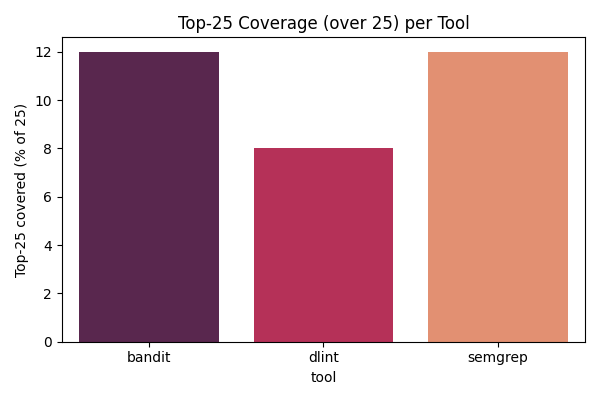
\includegraphics[width=\textwidth]{coverage_over_top25.png}
    \caption{Top‑25 coverage (over 25) per tool}
    \label{fig:cov_over_top25}
  \end{subfigure}\hfill
  \begin{subfigure}[b]{0.5\textwidth}
    \centering
    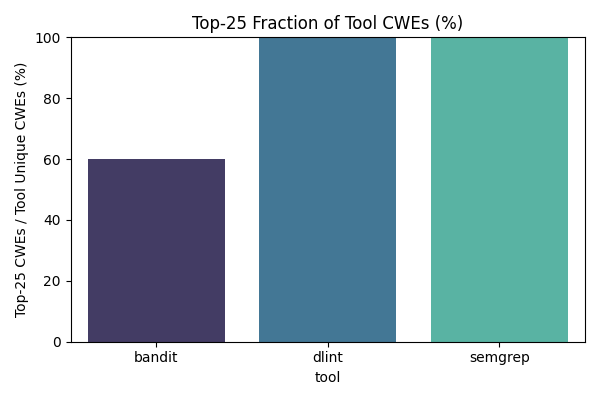
\includegraphics[width=\textwidth]{coverage_fraction_of_tool.png}
    \caption{Top‑25 fraction of tool CWEs (\%)}
    \label{fig:cov_fraction}
  \end{subfigure}\hfill
\end{figure}
  

% Optional: per-project IoU heatmaps (repeat/include for each project)
\subsection{Pairwise Agreement (IoU) Analysis}

\paragraph{IoU Definition:}
For tool sets \(S_{T_1}\) and \(S_{T_2}\) of unique CWE IDs, the IoU is:
\[
\mathrm{IoU}(T_1, T_2) = \frac{|S_{T_1} \cap S_{T_2}|}{|S_{T_1} \cup S_{T_2}|}.
\]
This is equivalent to the Jaccard Index on sets of detected CWE categories. 

\begin{algorithm}[H]
\caption{Compute pairwise IoU (tool-level and per-project)}
\begin{algorithmic}[1]
\REQUIRE consolidated CSV, OPTIONAL REPORT\_TOOLS list
\STATE tools $\leftarrow$ REPORT\_TOOLS if set else sorted(all tools in CSV)
\STATE tool\_sets $\leftarrow$ (for each tool: union of CWEs across projects)
\STATE IoU\_matrix $\leftarrow$ matrix(len(tools), len(tools))
\FOR{i=1 to len(tools)}
  \FOR{j=1 to len(tools)}
    \STATE A $\leftarrow$ tool\_sets[tools[i]]
    \STATE B $\leftarrow$ tool\_sets[tools[j]]
    \IF{A empty and B empty}
      \STATE IoU\_matrix[i,j] $\leftarrow$ 1.0
    \ELSE
      \STATE IoU\_matrix[i,j] $\leftarrow$ |A $\cap$ B| / |A $\cup$ B|
    \ENDIF
  \ENDFOR
\ENDFOR
\STATE \COMMENT{Repeat same per-project by building tool sets restricted to each project}
\end{algorithmic}
\end{algorithm}

\begin{figure}[H]
  \centering
  \begin{subfigure}[b]{0.33\textwidth}
    \centering
    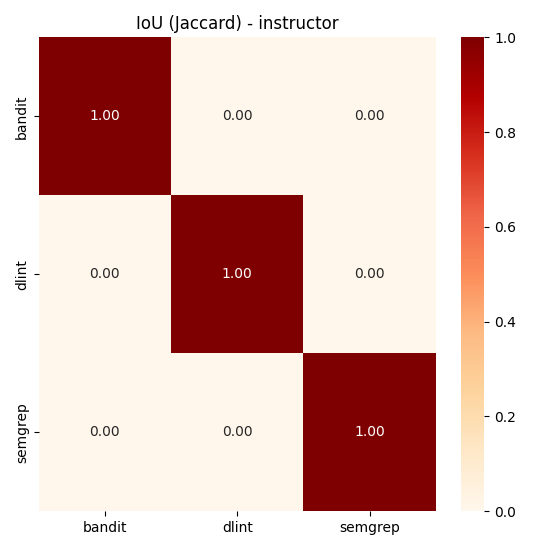
\includegraphics[width=\textwidth]{instructor_iou_heatmap.png}
    \caption{Instructor: IoU}
    \label{fig:iou_instructor}
  \end{subfigure}\hfill
  \begin{subfigure}[b]{0.33\textwidth}
    \centering
    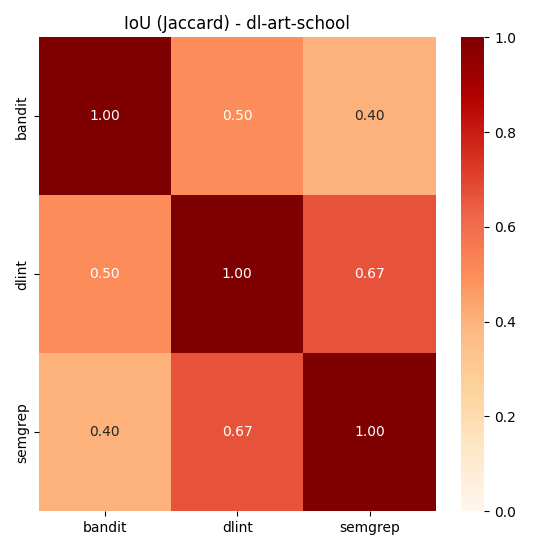
\includegraphics[width=\textwidth]{dl-art-school_iou_heatmap.png}
    \caption{dl-art-school: IoU}
    \label{fig:iou_dlart}
  \end{subfigure}\hfill
  \begin{subfigure}[b]{0.33\textwidth}
    \centering
    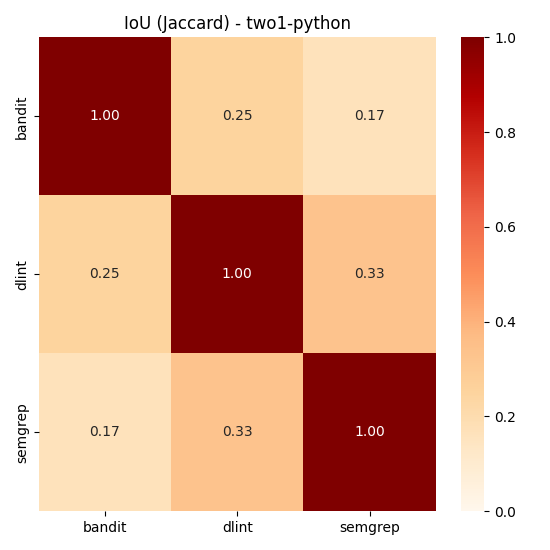
\includegraphics[width=\textwidth]{two1-python_iou_heatmap.png}
    \caption{two1-python: IoU}
    \label{fig:iou_two1}
  \end{subfigure}
  \caption{Per‑project IoU (Jaccard) heatmaps: empty entries indicate no findings for that tool/project pair.}
  \label{fig:per_project_iou}
\end{figure}

\begin{figure}
  \centering
  \begin{subfigure}[b]{0.5\textwidth}
    \centering
    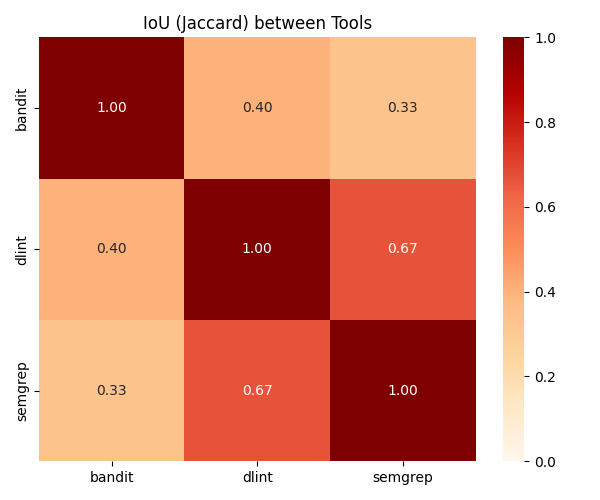
\includegraphics[width=\textwidth]{iou_heatmap.png}
    \caption{IoU (Jaccard) heatmap between tools}
    \label{fig:iou_heatmap}
  \end{subfigure}
  \caption{Tool‑level CWE coverage and IoU visualizations for the selected tools.}
  \label{fig:tool_coverage_and_iou}
\end{figure}

\subsubsection{Interpreting the IoU Matrix}

IoU (0–1) quantifies set overlap of CWE categories between tools. High IoU (e.g., >0.6) means the tools are largely redundant; semgrep vs dlint is the strongest overlap here $(\approx 0.67)$. Moderate IoU (around 0.3–0.5) shows partial overlap and useful complementarity (bandit vs dlint $\approx 0.40$; bandit vs semgrep $\approx 0.33$). Low IoU indicates tool‑specific coverage that increases the union when combined. Empty per‑project heatmap cells mean the tool reported no CWE‑tagged findings for that project.

Use IoU to pick pairs that balance non‑redundancy with meaningful Top‑25 contribution.

\subsubsection{Which tool combination maximizes CWE coverage?}

Heuristics: compare union sizes $(\|S_a \cup S_b\|)$ and marginal Top‑25 gains when adding a tool.

Summary for this dataset:
\begin{enumerate}
  \item Best single (Top‑25 oriented): semgrep or dlint (both have high fraction of their CWEs in Top‑25).
  \item Best pair: semgrep + bandit; semgrep is broad, bandit adds complementary categories (e.g., CWE‑338 / CWE‑428).
  \item Best trio: semgrep + bandit + dlint; yields the largest union and therefore the highest overall coverage, with diminishing marginal returns from dlint.
\end{enumerate}

Recommendation: run semgrep + bandit for a cost‑effective, high‑coverage baseline; add dlint when you need extra recall or confirmation for command‑injection/shell issues. Recompute IoU after changing rules/projects or tool versions.

% \section{Analysis and Discussion}
% \subsection{Coverage Insights}
% Summarize which tool has the broadest CWE coverage, and discuss Top-25 coverage differences. Note any domain/language biases or rule-set strengths that explain variance. 

% \subsection{Similarity and Diversity}
% Interpret IoU values: high IoU indicates overlapping detection patterns; low IoU suggests complementary detection capabilities. Identify pairs or combinations that improve coverage. 

% \subsection{Maximizing Coverage}
% State the best two-tool and three-tool combinations for maximizing CWE and Top-25 coverage across projects, with justification from the results. 

% \section{Threats to Validity}
% Discuss version differences, configuration parameters, buildability of targets, and language coverage limitations that may affect results. 

% \section{Reproducibility}
% Provide exact tool versions, commands, and configuration summaries (e.g., rules enabled, confidence thresholds), plus hardware/OS details and execution dates. 

% \begin{table}[H]
% \centering
% \caption{Reproducibility: Commands and Versions}
% \begin{tabular}{@{}ll@{}}
% \toprule
% Tool & Command / Version \\
% \midrule
% T1 & \texttt{TODO command} / vX.Y.Z \\
% T2 & \texttt{TODO command} / vA.B.C \\
% T3 & \texttt{TODO command} / vM.N.P \\
% \bottomrule
% \end{tabular}
% \end{table} 


\subsection{References}
\begin{itemize}[itemsep=0em, topsep=0pt]
    \item Lecture 6 slides: \href{https://drive.google.com/file/d/1OMsoLPEgdlNIqyNxAHWlhF7YjaNRAywQ/view}{here}
    \item Lab Assignment 6 document: \href{https://drive.google.com/file/d/1kuFDbnKFp2hOZsSrbkbHoyNt9NNvcMux/view}{here}
    \item SAST paper (FSE 2023): \url{https://sen-chen.github.io/img_cs/pdf/fse2023-sast.pdf}
    \item Static Analysis Tools List: \url{https://github.com/analysis-tools-dev/static-analysis}
    \item Jaccard Index (Wikipedia): \url{https://en.wikipedia.org/wiki/Jaccard_index}
\end{itemize}
